\documentclass[a4paper,11pt]{report}
\usepackage[a4paper, total={6in, 9in}]{geometry}
\usepackage{cite}
\usepackage{graphicx}
\usepackage{wrapfig}
\usepackage{appendix}
\usepackage{chngcntr}
\usepackage{caption}
\usepackage{float}
\usepackage{hyperref}

\counterwithout{figure}{chapter}

%%%%  Add some length to the page, as margins always seem too big.  
\addtolength{\topmargin}{-.25in}

\begin{document}

%%%%  Number the initial front matter with roman numerals
\pagenumbering{roman}


%%%%  TITLE PAGE
%%  Here are the elements that make up the title page of the document.  

\thispagestyle{empty}

\title{\LARGE
ASDA Stocking Support System (Xpire)}

\author{
Luke Michael Towell
\\    \\    \\
Dissertation
\\    \\
Submitted to 
\\    \\    \\ 
The University of Liverpool
\\    \\
\\    \\
in partial fulfilment of the requirements
\\
for the degree of 
\\     \\
MASTER OF SCIENCE
\\     \\    \\    \\
}


%%  Fill in a date here if you want, or comment out the line below and
%%  the current date will be automatically inserted for you.  
\date{}


\maketitle


%%%%  ABSTRACT
\chapter*{\center Abstract}

The aim of the project is to create an application which enables ASDA colleagues to identify
and inform colleagues of which items within their fresh departments are going out of date and
need to be marked down or could potentially be provided to food shelters. The software system produced by this project will make use of mobile technology,
 backend web services and database stored procedures in order to analyse and inform colleagues which items are scheduled to go 
out of date on which date and then informs colleagues to go and reduce the products. This application
will be used throughout ASDA stores by colleagues on a daily basis and could produce a significant
cost saving and waste reduction.
\\
\\
The final products of this project will be a system of applications which will be ready for deployment
into an ASDA store in the future. The requirements and periodic demoing of the produced solution will
be provided to ASDA technology colleagues throughout the period of the project.
\\
\\
More writing about the evaluation of the project and the final outcomes. 
\newpage

\chapter*{Code Repositories}
As this project has been completed multiple code repositories have been created for each of the applications.
Each code repository contains a README.md file which provides guidance on how to run each of the applications locally on a machine. Due to the fact that all of the application have been written on a Macbook Air they have not been tested on any other Operating Systems so there may be further set up required if not running on MacOS.

\section*{Front End Applications}
\subsection*{Mobile application}
The React Native code repository - \url{https://github.com/luketowell/xpire-mobile-app}
\subsection*{Web Application}
The React code repository - \url{https://github.com/luketowell/xpire-web-application}

\section*{Back End Services}
\subsection*{Web Services}
The Java Spring-Boot repository - \url{https://github.com/luketowell/xpire-web-services}
\subsection*{Database Scripts}
All Database scripts including create and drop scripts - \url{https://github.com/luketowell/xpire_db_scripts}

\section*{Accompanying Reports}
\subsection*{Design \& Specification}
The initial report outlining the design and specification of the project. - \url{https://github.com/luketowell/COMP702-Project}
\subsection*{Final Report}
The final report which summarises project progress - \url{https://github.com/luketowell/comp702-finalReport}

%%%%  STUDENT DECLARATION ON PLAGIARISM
\chapter*{\center Student Declaration} 

I confirm that I have read and understood the University's Academic Integrity Policy.

I confirm that I have acted honestly, ethically and professionally in conduct leading
to assessment for the programme of study.  

I confirm that I have not copied material from another source nor committed plagiarism
nor fabricated data when completing the attached piece of work.  I confirm that I have 
not previously presented the work or part thereof for assessment for another University
of Liverpool module.  I confirm that I have not copied material from another source, nor
colluded with any other student in the preparation and production of this work.  

I confirm that I have not incorporated into this assignment material that has been 
submitted by me or any other person in support of a successful application for a 
degree of this or any other university or degree-awarding body.  

\vspace*{1in}

\noindent SIGNATURE \verb!______________________________________!

\noindent DATE \hspace*{.4in}  \today

\vspace*{1in}

%%  NOTE ABOUT CONFIDENTIAL MATERIAL  
%%     Students who need to keep their dissertation confidential should uncomment
%%     the following sentence on this same page.  This will preclude the dissertation 
%%     from being placed in the University Library.  Students that submit work that 
%%     isn't confidential should leave this line commented out.  

% This dissertation contains material that is confidential and/or commercially
% sensitive. It is included here on the understanding that this will not be revealed to 
% any person not involved in the assessment process.  


\newpage

%%%%  ACKNOWLEDGMENTS
%%%%    A section for Acknowledgments, should you want one.



\newpage


%%%%  TABLE OF CONTENTS  
%%%%      Usually the following command will give you the formatting you want.  

\tableofcontents


%%%%  Turn page numbering back to arabic.  This also resets the numbering
%%%%  to begin again at page 1.  

\pagenumbering{arabic}

%%%%  INTRODUCTION

\chapter{Introduction}\label{chap:intro}

\section{Summary of Project Proposal}

\subsection{Problem Statement}\label{sec:problem}
The aim of this project is to design an application and waste management system which is able
to inform store managers and store colleagues on which items of stock are going out of date or are
close to going out of date on the shop floor. This stock will then either be marked 
down on the shop floor in order to be sold on the day or will be identified as able to be donated to other charitable
causes within the local community as part of the ASDA commitment to engage and assist in the local community.
\\
\\
The key goals of the developed system are to include:
\\
- An application which will direct colleagues to which items need to be marked down.
\\
- A reduction in store colleague hours spent in store manually marking down products.
\\
- Stock which is wasted will be reduced and identified for redistribution.
\\
\\
These goals will be assessed by peer review of colleagues in ASDA. I am also aiming to 
deploy the application in a live ASDA store with the aim of it being used in a live environment.
If I am able to deploy a POC into a live store then I will also assess the success of the 
application by comparing the product waste prior to usage in store against the wastage from 
the time that the application is used in store. 

\subsection{Project Methodology}
The methodology that I have chosen to implement for my project was a scrum agile methodology
which involved breaking the project down into smaller requirements which needed to be completed in 
iterations of development spread over the 8 weeks I developed my project in.  
\\
\\
The project included the management and development of multiple application features. Each of the features were 
detailed and documented on a Trello\cite{trello} kanban board (See Figure~\ref{fig:kanbanBoard}). 
As can be seen in Figure 1 the kanban board is broken down into "To Do", "Doing" and "Done" swim lanes.
\begin{figure}[H]
    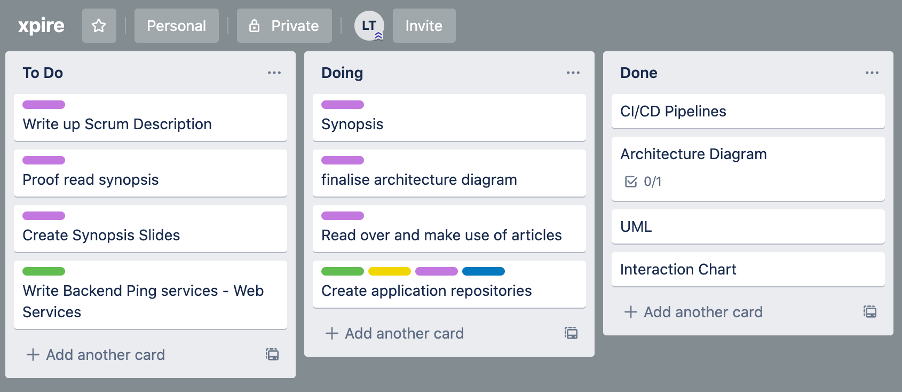
\includegraphics[width=\linewidth]{./assets/images/Kanban-board.png}
    \caption{Xpire Kanban Board}
    \label{fig:kanbanBoard}
\end{figure}

In Figure~\ref{fig:kanbanBoardFinal} you can see the updated Kanban board as I have been working on the project and moving the different requirements across the board as they have progressed.

\begin{figure}[H]
    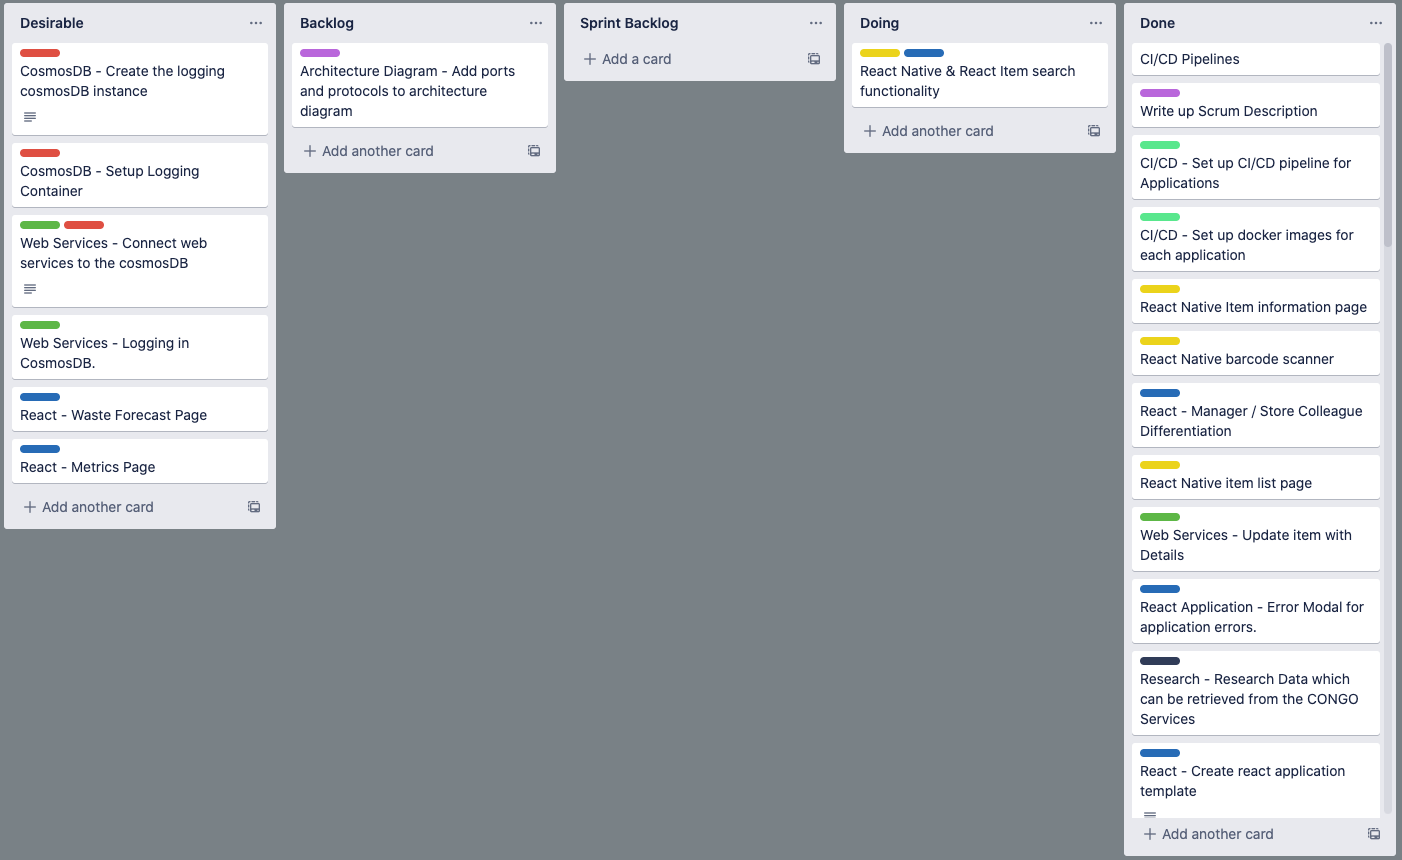
\includegraphics[width=\linewidth]{./assets/images/Kanban-2.png}
    \caption{Xpire Kanban Board - Towards completion of project.}
    \label{fig:kanbanBoardFinal}
\end{figure}

Since starting the project there have been some small changes to the way I used the Kanban board which are noticable in Figure~\ref{fig:kanbanBoardFinal}.
I have added a column to the board titled "Desirable", these are features that I have identified as being nice to have for the
project which essentially means that they are not essential to the project but could potentially add benefit if I have time to develop them.
\\
\\
I have also added labels to each of the cards so that I am easily able to identify which cards relate to each part of the application.
This has made it easier to look up which cards need working on and which features still require development. 


\chapter{Background}

At the moment sustainability and environmental responsibility are very prevelant in our day
to day lives. This ranges from the recycling which is carried out by all councils across
england to the protests and activism that takes place all across the UK by groups such 
as The Extinction Rebellion. There are regularly discussions in the media about the impact
that society and our daily habits are having on the world that we live in and what we need
to do to attempt to repair and improve our environmental impact. Wrap (Waste \& Resources Action Programme) \cite{wrapvision}
is a charity which is focused on raising public awareness of the various types of waste throughout the UK
in order to improve the use of resources in a more efficient way and to develop more sustainable products.
One of the focuses of WRAP is the food industry, WRAP highlights that approximately one third of global food
is wasted which equates to an economic loss of approximately \$984 billion globally and above £19 billion in the UK alone \cite{wrap-food-drink}.
\\
\\
It is largely accepted that we all have a part to play in assisting and improving the environment
of the planet and this is especially true for large corporations and businesses. 
\\
\\
ASDA has also focused on various schemes to be a more environmentally conscious retailer. 
These can include working with FareShare \cite{asda-food-waste} or reducing their plastics. 
\\ 
\\  
As part of the further research into the previous work others have done that is similar to my project 
I have looked for potentially similar applications which offer similar functionality to users. 
Below is an outline of the applications and a comparison against the functionality that they
offer against what my app will capable of.

\subsubsection{Too Good To Go}
Too Good To Go is an application which users are able to install on their devices.
The app displays to the user businesses which are offering their surplus food for a reduced price.
The user simply has to visit the business which is selling its reduced stock in the form of a "Magic Bag" \cite{too-good-to-go}.
\\
\\
When looking at Too Good To Go there are certainly similarities to the application that I am going to 
produce with regards to the aim of reducing waste however the main difference is that Too Good To Go 
has a focus on being the central hub for retailers to advertise their reduced produce where as the application
 I intend to produce will highlight to the user which items are going out of date. 

\subsubsection {Totalctrl}
TotalCtl is an application focused on inventory management and identifying when items are going to go out of
date which then allows the retailer, restaurant, cafe or other business to either dispose or reduce their products.
TotalCtl enables management via dashboards, graphing and alerting and is very similar application to what I am to produce\cite{totalctrl}.
\\
\\
The main difference I have identified between totalctl and my proposed solution
is that total control requires the user to upload invoices from suppliers when
items are delivered so that it can maintain its record keeping. My application 
on the other hand will make use of internal ASDA data stores, these are automatically
updated and will also enable the store to monitor stock without colleagues having to
manually enter invoices into the system.
\\
\\
Obviously the other key difference between my application and the applications discussed previously
is that my application will only deal with identifying waste that is going to go out of date within ASDA stores.
Once the stock is identified then it will be up to the colleague to decide what is done with that store following ASDA policy.
\\
\\
The main benefit of my application is that it is built bespoke for ASDA architecture and makes
use of current systems and architecture ensuring that from the beginning the application will 
work inside the ASDA ecosystem without the need for any extra development costs to make use of
a third party application. 

\subsection{Project requirements gathering}

As well as looking at examples of other applications which offer similar functionality to my proposed
 application I also gathered requirements from ASDA employees who are familiar with the requirements 
 of the project. Each of these requirements where broken down into development cards and documented on
  the project Trello board. Each card contains the aim of the card, the requirement that the development
   will provide and the functionality which will be available once the card has been completed. 

%    TODO: insert a figure of a well documented card

% TODO: Insert notes from discussion with Philippa to document the gathering of requirements from members of the ASDA project management staff. 

% TODO: Insert potential notes from confluence. 

\chapter{Ethical Use Of Data}
\section {Data Used Within The Application}


% TODO: CITE SPECIFICATION AND DESIGN DOCUMENT
\chapter{Design}
The aim of this project from the outset was to create a software system which makes use of multiple applications
 to give the in store user a clean and easy to use way of managing in-store waste. In the following chapter I 
 discuss what has been produced and what I will discuss in my dissertation.

\section{User Interface Design}

As part of the development of the system a key to ensuring the ease of use of the application was to take care and attention when
designing the user interface of the different applications. In order to do this I made use of Balsamic\cite{balsamiq} in order to design the user
interface of both the mobile and web applications. Figure~\ref{fig:UIDesignExample} shows an example of the 
interface design in Balsamiq and the final user interface that was produced. 

\subsection{Mobile Application User Interface Design}

\begin{figure}[H]
    \centering
    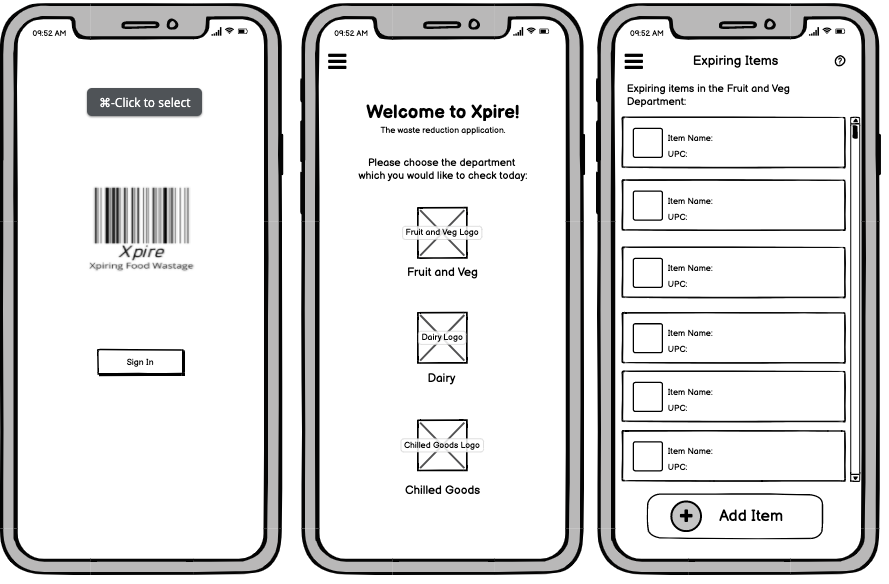
\includegraphics[width=11cm]{./assets/images/uiDesign-example.png}
    \caption{Example of the User Interface designs.}
    \label{fig:UIDesignExample}
\end{figure}


\subsection{Web Application User Interface Design}

\section{Database Design}
One of the features of the system which probably took the most amount of time and research was the database.
The database schema below (See Figure ~\ref{fig:DBSchema}) shows the final design of the database including foreign key relationships, primary keys and tables.

\begin{figure}[H]
    \centering
    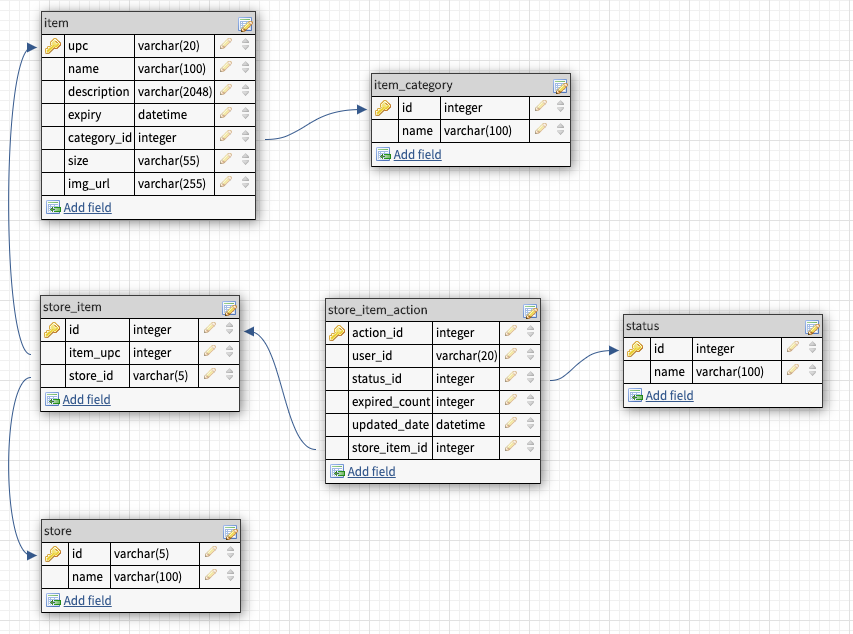
\includegraphics[width=12.5cm]{./assets/images/Database-Schema.png}
    \caption{Final database schema.}
    \label{fig:DBSchema}
\end{figure}

In my dissertation I will go into more information about the challenges which arose whilst I was implementing the database  and the considerations
which I needed to make in order to ensure that the design was suitable for the software system.


\chapter{Realisation}
In the following sections I will discuss the applications which where developed as part of the Xpire system.

\section{Mobile Application}
The mobile application of Xpire is the main part of the system which is used by the front of house store colleagues who are working on the shop floor.
The application has been written using the React-Native JavaScript framework which means that it is compatible with both android and IOs operating systems.
This means the app can be used on both in store devices as well as colleague and managers personal devices as part of the BYOD (Bring Your Own Device) scheme. 

The application is capable of communicating with the back end web services via Restful CRUD requests which ensures that all user data is as up to date as possible.
The application also includes a barcode scanner which enables users to easily scan items rather than entering relevant barcode numbers for items that they want to look up. 
\\
\\
Figure ~\ref{fig:IOSScreenshots} shows an example of the IOs version of the apps user interface. These screenshots can be directly compared against Figure ~\ref{fig:UIDesignExample}
 to show how the designs of the application have been implemented in the final versions of the application.

\begin{figure}[H]
    \centering
    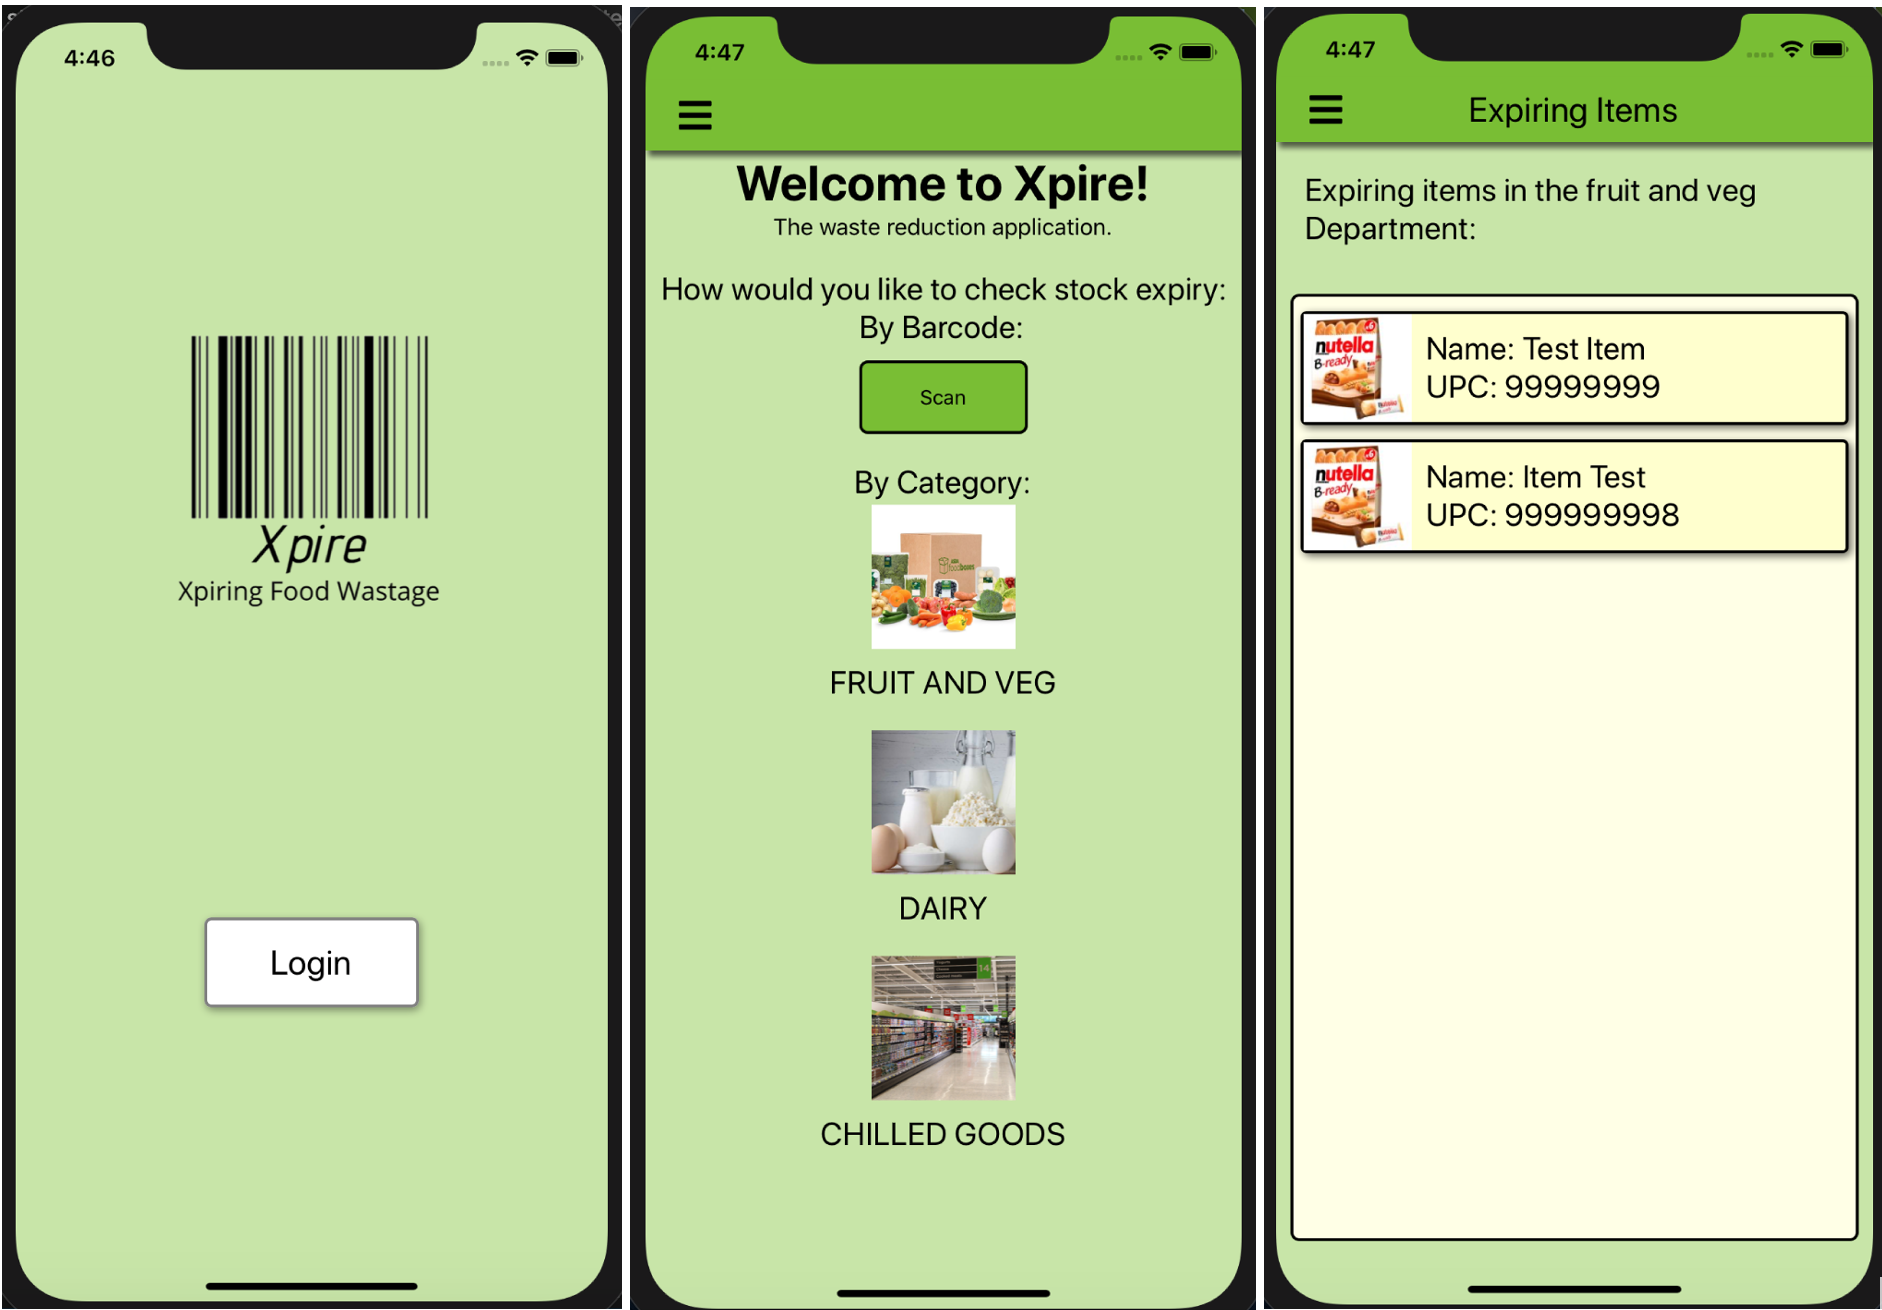
\includegraphics[width=10cm]{./assets/images/appUI.png}
    \caption{Screenshots of the IOs mobile application.}
    \label{fig:IOSScreenshots}
\end{figure}

\section{Web Application}
The web application of the system has been written in the React JavaScript framework. The functionality of the application is largely the same as the mobile application however because the web view is available on a larger screen size I have used this to my advantage and included slightly more information for the user. 
The functionality for the web application also differs slightly by offering a different view for managers who are able to view the items and information of other stores as well as their own. 
Figure ~\ref{fig:WebUi} is a screen shot of the application which includes the functionality to change stores.

\begin{figure}[H]
    \centering
    \frame{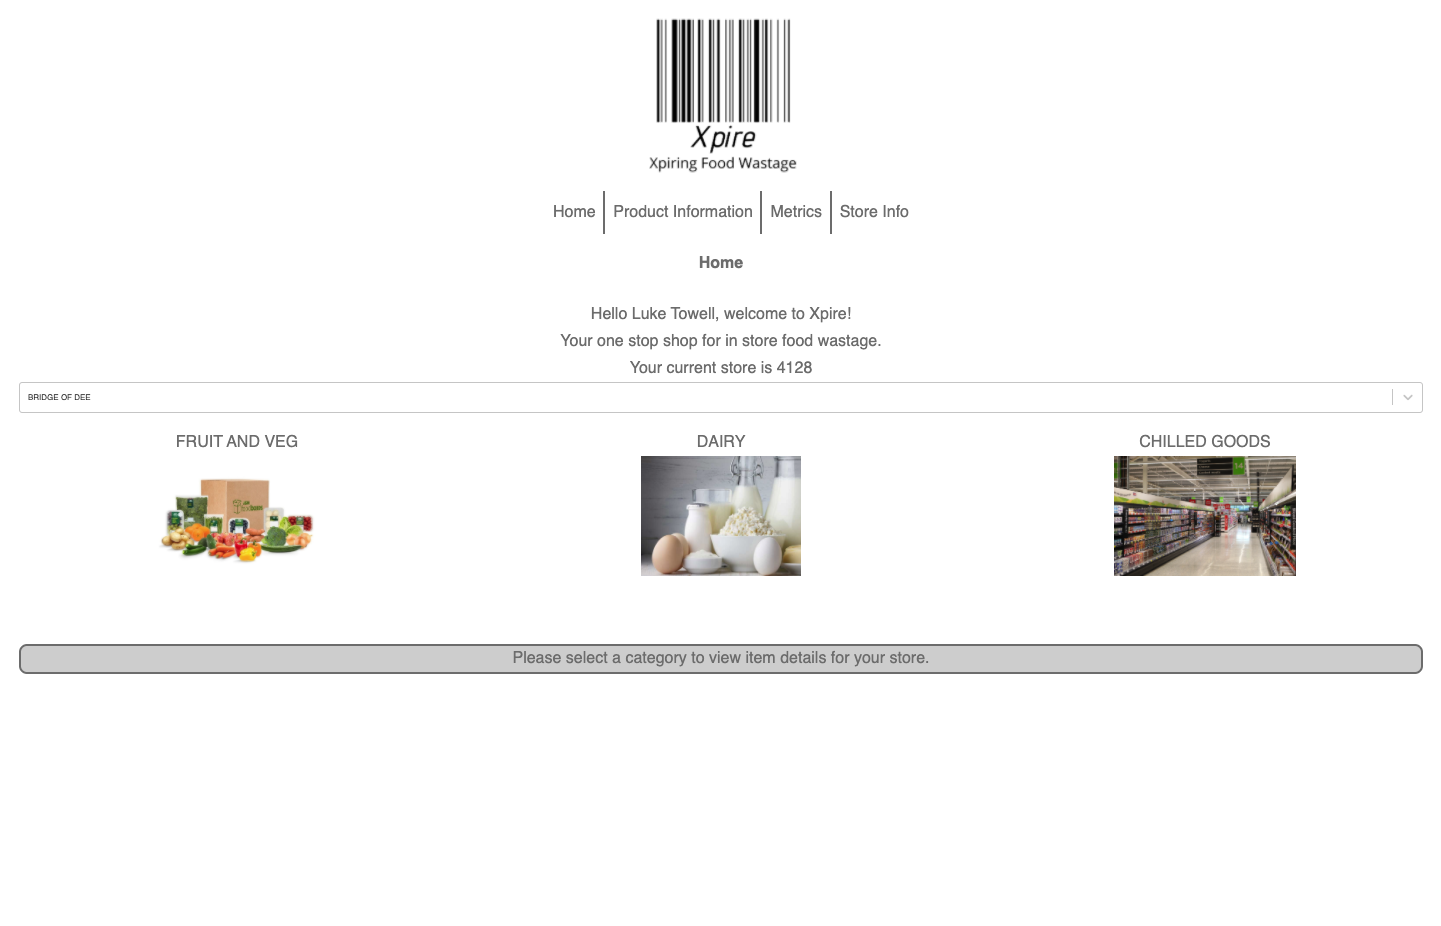
\includegraphics[width=10cm]{./assets/images/webUI.png}}
    \caption{Screenshots of the initial landing page of an authenticated user.}
    \label{fig:WebUi}
\end{figure}

\section{Web Services}
In order to manage the communication between the front end applications and the database I have written web services in Java using the Spring Boot framework. 
The application has been designed using the "repository pattern" which is discussed in the Gang of Four Book, Design Patterns: Elements of Reusable Object-Oriented Software\cite{gamma1994design} which creates an interface between the front end user and the database.

In my dissertation I plan on describing how the web services have been written and the technology which has been used in order to ensure that the services are easy to use and deploy.

\section{Testing of the Applications}

\chapter{Evaluation}
\section {Successes of the project}
Overall based on the aims of the project I believe that the project has been a success. I have produced a system which comprises of several different applications whilst making use of several different programming languages and design concepts. 
 Whilst there have been issues over the course of the project I have received positive feedback from the Project Manager colleagues within ASDA who have been overseeing the project.
I believe that with more time to go through the correct security checks that are mentioned in the challenges section of this report that the project would demonstrate a reduction in 
colleague time spent checking waste stock and an overall increase in colleague performance. 
\\
\\
In the dissertation which will follow this report I plan on going through the individual aspects of the project and identifying how I believe that they have been positively addressed.

\section {Challenges of the Project}
Throughout the project there have been issues which have arisen an the solution has been developed. In the early stages of the project it was identified that due to data security and authentication security utilised by ASDA I would be unable to make use of data and Authentication systems. This has presented various different issues which include:
\begin{itemize}
    \item Data availability
    \item User Authentication
    \item Application and Database hosting
    \item Store Usage
\end{itemize}

All of these issues have been over come or worked around in order to produce a working software system. Each of the Issues listed above will be discussed in more detail along with the relevant work arounds in the dissertation of this project.


\section{Colleague Feedback}
Unfortunately due to the limitations that have been mentioned above and will be expanded upon in my dissertation I was unable to place the system into a production ASDA store.
Because of this I have had to re-assess how I will gather feedback on the system. The project will now be assessed by ASDA colleagues and managers based on demonstrations of the application within different user scenarios. 
In my dissertation I will discuss the feedback which I receive and summarise the positives and potential improvements that the ASDA colleagues raise in their feedback.

\chapter{Learning Points}
% Java Spring Boot
% Repository Pattern
% Design Patterns

% SQL and Database integrations
% Table Relationships
% Normalisation

% Docker and Containerisation
% Organisation
% Time Management
% Project structure

\chapter{Professional Issues}

\chapter{Conclusions}
% How do I feel the application has been completed?
% What would it take to put the application into production
% What extra work could be completed in order to finish the application?
% Potential for project expansions?

%%%%   REFERENCES

%%%%  Section for references, using the \bibitem directive to 
%%%%  specify labels used to cite sources in the document.  

\addcontentsline{toc}{chapter}{Bibliography}
\bibliography{bibliography}
\bibliographystyle{plain}


%%%%   APPENDICES
\newpage
\addcontentsline{toc}{chapter}{Appendices}
\begin{appendix}
\end{appendix}

\end{document}
